\documentclass[11pt]{article}

\title{{\Large Exact, Discrete, Multi-objective Optimization} \\ ECE498A Project Specification}
\author{Joseph Hong, Chris Kleynhans, Ming-Ho Yee, Atulan Zaman \\
        \{yshong,cpkleynh,m5yee,a3zaman\}@uwaterloo.ca}

% For definitions
\usepackage{amsthm}
\theoremstyle{definition}
\newtheorem{mydef}{Definition}

% TikZ is what lets us draw graphics
\usepackage{tikz}
\usetikzlibrary{shapes.multipart,positioning,arrows}

\usepackage{graphicx}
% For table
\usepackage{float}

%For table caption
\usepackage{caption}

%For limited depth table of content
\usepackage{titletoc}


%Declaring new column types for multiline columns
\usepackage{array}
\newcolumntype{L}[1]{>{\raggedright\let\newline\\\arraybackslash\hspace{0pt}}m{#1}}
\newcolumntype{C}[1]{>{\centering\let\newline\\\arraybackslash\hspace{0pt}}m{#1}}
\newcolumntype{R}[1]{>{\raggedleft\let\newline\\\arraybackslash\hspace{0pt}}m{#1}}

\begin{document}
\maketitle

\tableofcontents
% Sets table of content of depth 1
\addtocontents{toc}{\setcounter{tocdepth}{1}}


\newpage

\section{Motivation}\label{sec:motivation}
Multi-objective optimization is a widely researched area of computer
science that focuses on finding solutions to problem definitions with
respect to given objective realization constraints. Computing such
solutions is extremely resource intensive, and the computation time
grows exponentially with the number of optimization variables.

The nature of our work in scientific terms is called \textit{exact,
discrete multi-objective optimization}. Multi-objective optimization
(MOO) is the process of computing the most optimal solutions given a
goal and a set of constraints.

\textit{Multi-objective} means that there are multiple metrics that
must be optimized over. Thus, more than one optimal solution may be
found that satisfies the various optimization goals.

\textit{Exact} in the context of our problem indicates that all
solutions computed by the algorithm are Pareto-optimal. Informally,
this means none of the solutions can be improved without compromising
at least one other optimization goal. Heuristic approaches for
multi-objective optimization do not guarantee that all their solutions
are Pareto-optimal.

\textit{Discrete} indicates that our optimization algorithm only
addresses discrete, or combinatorial, input data. The algorithm does
not accept continuous optimality conditions.

One simple example of a multi-objective optimization problem is the
satellite scheduling problem. In this problem~\cite{ref:nasa11}, NASA
must determine the best possible satellite launch schedule that
maximizes scientific value. Each satellite has a different cost,
purpose, and value to a different scientific community. In this
problem, the constraints for NASA are such things as resource
limitations and launch ordering constraints.

Moolloy~\cite{ref:Rayside09} is a tool introduced by the MIT Computer
Science and Artificial Intelligence Laboratories that solves
multi-objective optimization problems. It also has a GUI that lets the
user specify the constraints and objective conditions, as well
graphically view the Pareto-optimal solutions computed by the
algorithm. The underlying algorithm, called the \textit{guided
improvement algorithm}, is capable of solving small problems. However,
its scalability is greatly limited by the time it takes to compute
solutions for large problems, since the algorithm must make multiple
calls to a SAT solver.

Therefore, our work will focus on increasing the performance of
Moolloy, while ensuring the algorithm continues to perform correctly.

%%%%%%%%%%%%%%%%%%%%%%%%%%%%%%%%%%%%%%%%%%%%%%%%%%%%%%%%%%%%%%%%%%%%%%%%

\section{Related Work}\label{sec:related_work}

The \textit{guided improvement algorithm} was described by Rayside,
Estler, and Jackson~\cite{ref:Rayside09} in 2009. In their paper, they
also conducted a literature survey on related work. Rayside et al.\
found that most multi-objective problems were concerned with continuous
variables, as opposed to discrete variables.

Furthermore, most of the research on multi-objective optimization they
found was focused on heuristic approaches, specific instead of general
solvers, extensions of single-objective solvers, or problems with only
two or three variables.

The guided improvement algorithm is an exact, discrete, general-purpose
solver. Furthermore, it is not an extension of a single-objective
approach. Rayside et al.\ identified a similar approach they call the
\textit{opportunistic improvement algorithm}, which was independently
discovered by Gavanelli~\cite{ref:Gavanelli02} and Lukasiewycz, Gla\ss,
Haubelt, and Teich~\cite{ref:Lukas07}. Notably, the guided improvement
algorithm produces intermediate Pareto-optimal results during its
computation.

Only three publications have cited the guided improvement algorithm
paper since it was published. One of them describes a spreadsheet-like
user interface, while the other two concern applications of the
algorithm. Thus, none of them are related to our work, which is
strictly to optimize the algorithm.

%\mbox{} to prevent line-breaking K-PPM
A more recent paper by Dhaenens, Lemesre, and Talbi ~\cite{ref:kppm}
proposes \textit{\mbox{K-PPM}}, an algorithm which can be parallelized.
However, the algorithm does not produce intermediate Pareto-optimal
results.


%%%%%%%%%%%%%%%%%%%%%%%%%%%%%%%%%%%%%%%%%%%%%%%%%%%%%%%%%%%%%%%%%%%%%%%
\section{Intended Users \& Research Value}\label{sec:research_val}
Multi-objective optimization problems appear in may different fields.
By improving the performance and scalability of the algorithm, we will
enable its usage for problems with larger input spaces. We have
identified potential case studies from three different fields who shall directly benefit from the work of this research:
aerospace, civil engineering, and software engineering.

\subsection{Aerospace}\label{sec:aerospace}
Every ten years NASA performs its decadal survey to determine the
satellite launch schedule for the next decade~\cite{ref:nasa11}.
Multi-objective optimization can be used to determine a schedule that
maximizes scientific value to different scientific communities while
minimizing cost. Furthermore, many different constraints must be
satisfied. For example, one satellite may depend on another, or a
satellite may need to match a specific timeline.

\subsection{Civil Engineering}\label{sec:civil_eng}
Dr.\ Bryan Tolson, a civil engineering professor from the University of
Waterloo, has identified a number of multi-objective optimization
problems in his research. Currently, the problems are solved using
heuristic methods, in other words, genetic algorithms. As discussed
earlier, these methods do not guarantee that their solutions are
Pareto-optimal. One of Dr.\ Tolson's problems is to determine the
optimal type, quantity, and arrangement of materials to line a landfill
in order to minimize seepage, while keeping cost minimal.

\subsection{Software Engineering}\label{sec:soft_eng}
We will be collaborating with Rafael Olaechea, a graduate student at
the University of Waterloo who is interested in the \textit{software
product lines} problem~\cite{ref:Olaechea12}. This problem involves
determining which modules should be included in the software for an
embedded device. Each module can perform different functions, which may
conflict with other modules. Additionally, each module will have a
different cost in terms of code size and performance metrics.
Therefore, the problem is to determine an optimal set of modules for a
device, while satisfying the functionality constraints.

\subsection{Potential Users}\label{sec:potential_users}
Besides the specific use cases mentioned above, the concept of multi-objective optimization is useful in many other fields of engineering and with the success is scalability it will be applicable to many other domains, eg.\ the domain of scheduling problems similar to the aerospace problem which can be extended to more domains.

%%%%%%%%%%%%%%%%%%%%%%%%%%%%%%%%%%%%%%%%%%%%%%%%%%%%%%%%%%%%%%%%%%%%%%
\section{Overall Description}\label{sec:overall_desc}
The overall description of the system is introduced by first declaring some of the technical definitions, acronyms and abbreviations that will be used throughout the document and the feature descriptions. It also introduces some of the technical terms used in the write-up for users not familiar in this domain. Followed by the definitions, a system block diagram is presented to illustrate the interaction between the different elements in the system. A table of description is also provided for each node in the block diagram.

\subsection{Definitions, acronyms, abbreviations}\label{sec:def}
% Usually for domain-level definitions
% Explain any naming conventions you develop to help you write the
% document
% Explain any notational conventions for any deviations from the
% standard UML notation

% Definitions
\begin{mydef}
A solution is said to be \textit{Pareto-optimal} if and only if it is
not \textit{dominated} by any other solution. A solution $a$ dominates
a solution $b$ if all metrics of $a$ are greater than or equal to their
corresponding metrics of $b$, and there exists some metric of $a$ that
is strictly greater than its corresponding metric of $b$.
\end{mydef}

\begin{mydef}
The set of all Pareto-optimal solutions is called the
\textit{Pareto front}.
\end{mydef}

\begin{mydef}
A \textit{multi-objective optimization (MOO) problem} is a problem with
multiple constraints, as well as multiple goals to optimize over.
\end{mydef}

\begin{mydef}
An \textit{exact} solution to a multi-objective optimization problem is
the Pareto front.
\end{mydef}

\begin{mydef}
\textit{Discrete} in this document means that there is a countable
number of configurations for every problem. This is in contrast to the
continuous case. A synonym for discrete is \textit{combinatorial}, but
we will only use the former term.  \end{mydef}

\begin{mydef}
By \textit{general-purpose}, we mean that Moolloy can solve any
multi-objective optimization problem, as opposed to a specific one.
\end{mydef}

\begin{mydef}
\textit{SAT}, or \textit{boolean satisfiability}, is a problem that
asks whether a given Boolean formula can be assigned values such that
its evaluation is true. In other words, it asks if a given Boolean
formula can be satisfied.
\end{mydef}

% Overall description of the system including general factors that
% affect the product and its requirements
%   Do not state specific requirements here instead provide a
%   background for those requirements.
\subsection{System Block Diagram}\label{sec:block_diag}
All multi-objective optimization problem models are first converted to relational models using the Alloy modelling language. As input, Moolloy takes a multi-objective optimization problem modelled in Alloy, and returns the Pareto front as an Alloy instance. Moolloy, as an extension of Alloy, is written in Java. Moolloy compiles the alloy models and compiles into an intermediate form which is passed to the Kodkod solver. Kodkod in turn takes the intermediate forms and compiles them into SAT formulaes which can be used to makes calls to an external SAT solver. The satisfiable instance produced by the solver is then returned to Kodkod, and Kodkod then reverse compile it to Alloy and solution is shown as an Alloy instance. Kodkod and the SAT solver are packaged with Moolloy.  Figure~\ref{fig:overview} depicts
the overall structure of Moolloy.

% TIKz diagram for block diagram

\begin{figure}[htbp]
  \centering
    \tikzset{>=latex}
    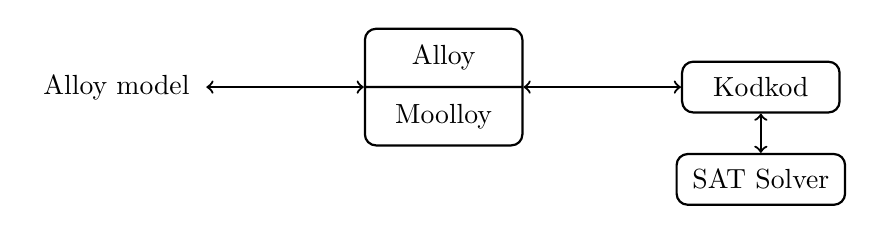
\begin{tikzpicture}[
      every node/.style={rectangle,thick,draw=black,text ragged,
                         rounded corners,inner sep=2mm,
                         text centered,minimum width=20mm},
      split/.style={rectangle split,rectangle split parts=2},
      double/.style={draw,thick,<->},
      single/.style={draw,thick,->},
    ]
      \node[draw=none] (model) {Alloy model};
      \node[split, right=2cm of model] (alloy) {
        \nodepart{one} Alloy
        \nodepart{two} Moolloy
      };
      \node[right=2cm of alloy] (kodkod) {Kodkod};
      \node[below=0.5cm of kodkod] (sat) {SAT Solver};
      \path(model) edge[double] (alloy);
      \path(alloy) edge[double] (kodkod);
      \path(kodkod) edge[double] (sat);
    \end{tikzpicture}
  \caption{Overview of Moolloy structure.}\label{fig:overview}
\end{figure}

We assume that all users are already familiar with multi-objective
optimization, including such terms as \textit{Pareto-optimal} and
\textit{Pareto front}. Furthermore, we assume users are familiar with
how SAT solvers are used to find these solutions. The user should also
be familiar with expressing the problem in Moolloy's domain specific
language, as well as interpreting the results.

Some technical details behind the components of the Moolloy system is provided in the table below.

% Uses manually defined column commands to allow multiline columns in latex tables

\begin{table}[H]
  \captionsetup{margin=30pt}
  \caption{Component Details}\label{component_details}
  \centering
  \begin{tabular}{l  L{7cm}  R{3cm}}
    \hline
    \multicolumn{1}{c}{\textbf{Item}} &
    \multicolumn{1}{c}{\textbf{Purpose}} &
    \multicolumn{1}{c}{\textbf{API}}\\
    \hline
      Alloy & Relational Modelling Language & Java, MIT License \\
      \hline	
      Moolloy & Alloy with multi-objective solver features & Java, MIT License \\
      \hline
      Kodkod & Compiles Alloy models to SAT formulaes to call SAT solver & Java, MIT License \\
      \hline
      SAT Solver & Accepts SAT formulaes from Kodkod, solves and reports solution & Many\\
    \hline
  \end{tabular}
\end{table}
 
%%%%%%%%%%%%%%%%%%%%%%%%%%%%%%%%%%%%%%%%%%%%%%%%%%%%%%%%%%%%%%%%%%%%%%
\section{Functional Requirements}\label{sec:func_req}
% Requirements and specifications
% UML and UI diagrams go in here
For this project, the functional requirements describe the research objectives of optimizing Moolloy. The criteria for optimizing Moolloy basically comes in two dimensions: Scalability and Speed. The basis for setting a benchmark in these criteria are explained below. These two are related, as significant improvements in speed will allow Moollloy to scale up and handle larger inputs.

\subsection{Speed}\label{sec:perf_speed}

Moolloy's algorithm works by making multiple calls to a SAT solver for
each multi-objective problem it must solve. These calls can be
classified as \textsc{sat} and \textsc{unsat} calls, where \textsc{sat}
calls can be satisfied, and \textsc{unsat} calls cannot be satisfied.
\textsc{unsat} calls are very expensive, while \textsc{sat} calls are
less expensive, since they terminate once a solution is found.

Our goal is to improve the speed at which Moolloy solves a problem.
This allows users to solve our current problems much faster. To
accomplish this goal, we aim to reduce the number of \textsc{sat} and
\textsc{unsat} calls.

From Rayside et al.'s paper~\cite{ref:Rayside09}, the twenty-five
variable, four metric knapsack problem takes approximately forty-five
hours to complete, in the process requiring 1,938 calls to the SAT
solver, where 814 were \textsc{unsat}. Our goal is to reduce this time
to under twenty-four hours.

\subsection{Scalability}\label{sec:perf_scale}

Because solving large problems is very expensive, there are many
real-world problems that simply cannot be solved at this time. We aim
to optimize Moolloy so that such problems are solvable.

\section{Non-Functional Requirement}\label{sec:nonfunctional}
These non-functional requirement are basically constraints that must considered during the development of the software project for proper software design practices and quality but are not part of the feature specifications.  These criteria avoid regression of the existing Moolloy system and support design compatibility.

\subsection{Design Constraints}\label{sec:constraints}

As Moolloy is currently implemented in Java, the new version must also
be implemented in Java. Furthermore, to maximize the utility of this
program, Moolloy must be able to build and run on any platform that
supports Java.

\subsection{Preventing Regresssion}\label{sec:regression}
We shall be working on a repository branch of the source code for Alloy and Kodkod which shall needs to prevent regression of existing features for it to be merged to the existing codebase therefore it is important to have proper use cases and continuous integration system while we work on the project.

%%%%%%%%%%%%%%%%%%%%%%%%%%%%%%%%%%%%%%%%%%%%%%%%%%%%%%%%%%%%%%%%%%%%%%%
\section{Risks \& Technical Feasibility}\label{sec:risks}
One risk in this project is that we may not be able to find good test
cases to evaluate our optimization techniques. Each problem is
different, and thus there are many possible routes for optimization.
Furthermore, significant domain knowledge may be required to properly
model the problems. This is why we are working with multiple
collaborators in different fields, to obtain both test problems and
relevant domain knowledge.

An unlikely risk for this project is that none of our techniques
provide satisfactory results in terms of performance. There is still
research value, although very little research impact, as there is very
little benefit to users.

%%%%%%%%%%%%%%%%%%%%%%%%%%%%%%%%%%%%%%%%%%%%%%%%%%%%%%%%%%%%%%%%%%%%%%%
\section{Costs}\label{sec:costs}
We estimate our expense to be around \$350 as a result of purchasing various tools and
services, as well as hardware infrastructure for our tests.
Table~\ref{tbl:costbreakdown} shows the total cost breakdown for our
project.

\begin{table}[H]
  \captionsetup{margin=30pt}
  \caption{Total cost breakdown}\label{tbl:costbreakdown}
  \centering
  \begin{tabular}{lr}
    \hline
    \multicolumn{1}{c}{\textbf{Item}} &
    \multicolumn{1}{c}{\textbf{Cost}} \\
    \hline
      Atlassian Bamboo (continuous integration and build system) & \$150 \\
      Atlassian HipChat (asynchronous communication platform) & \$150 \\
      Amazon EC2 Instances (cloud computing infrastructure) & \$50 \\
    \hline
    \textbf{Total} & \$350 \\
    \hline
  \end{tabular}
\end{table}





% Appendices
\appendix

%%%%%%%%%%%%%%%%%%%%%%%%%%%%%%%%%%%%%%%%%%%%%%%%%%%%%%%%%%%%%%%%%%%%%%
\section{Guided Improvement Algorithm}\label{app:impl}

This appendix outlines, at a high-level, how the \textit{guided
improvement algorithm} works. Rayside et al.~\cite{ref:Rayside09}
provide a more formal and detailed description in their paper.

First, Moolloy finds a solution that satisfies the constraints. Once
this solution is found, Moolloy finds a new solution that dominates the
previous one. Moolloy continues this process of finding new solutions
until no other dominating solution can be found---this last solution is
on the Pareto front, by definition.

Moolloy continues this process with new starting solutions (that are
not dominated by any previously discovered solution) until all
solutions on the Pareto front are found.

Thus, Moolloy makes a large number of calls to the underlying SAT
solver. These are extremely expensive calls, so the goal for optimizing
Moolloy is to reduce the number of calls to the SAT solver.

%%%%%%%%%%%%%%%%%%%%%%%%%%%%%%%%%%%%%%%%%%%%%%%%%%%%%%%%%%%%%%%%%%%%%%%%

\bibliographystyle{ieeetr}
\bibliography{specifications}


\end{document}
